\documentclass{article}
\usepackage{enumitem}
\usepackage{graphicx}
\usepackage{subcaption}
\usepackage{tikz}


\begin{document}

\section*{3D Reconstruction and dimention measurement}
Photogrammetry is essential for understanding and conserving aquatic ecosystems, particularly in coral reef research and species preservation. By converting 2D images into 3D models, it enables thorough ecosystem assessment and environmental monitoring. This technology provides vital insights into species behavior, contributing to informed conservation efforts and the sustainable management of aquatic habitats.

\subsection*{3D Reconstruction Procedures}
In order to reconstruct a 3D model of a specific object, Draven rotates around it while capturing a video that is then saved as a sequence of individual image frames. Subsequently, a Structure From Motion (SfM) algorithm is employed to analyze these image frames, identifying common visual features across the entire sequence. This process enables the estimation of the camera positions and orientations required to create a dense 3D model. The dense model comprises a collection of points representing these common visual features, effectively capturing the intricate details of the object's structure. Finally, to enhance the realism and appearance of the model, a texturing process is applied, effectively adding surface details and colors to produce a complete and visually accurate 3D representation, as specsified in Figure \ref{fig:reconstruction}.
\begin{figure}[h]
  \centering
  \begin{tikzpicture}
    % First figure
    \node[draw, rectangle, blue, fill=blue!20] (figure1) at (0,2) {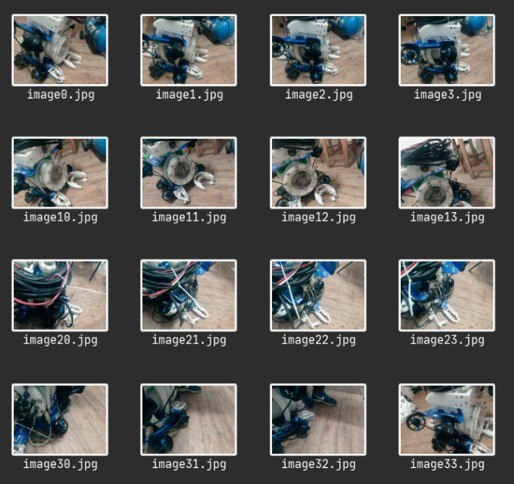
\includegraphics[width=0.3\textwidth]{"3d_task_figure2/input_images 2.jpg"}};
    \node[above=65pt, text width=100pt,align=center] at (figure1) {Samples from input images};
  
    % Second figure
    \node[draw, rectangle, blue, fill=blue!20] (figure2) at (4,2) {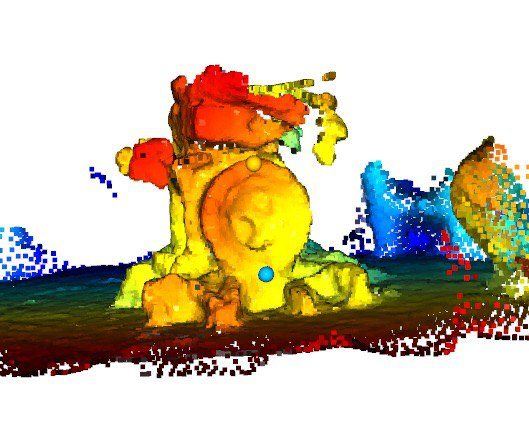
\includegraphics[width=0.25\textwidth]{3d_task_figure1/reference 2.jpg}};
    \node[above=50pt, text width=100pt,align=center] at (figure2) {Dense reconstruction Output};
  
    % Third figure
    \node[draw, rectangle, blue, fill=blue!20] (figure3) at (8,4) {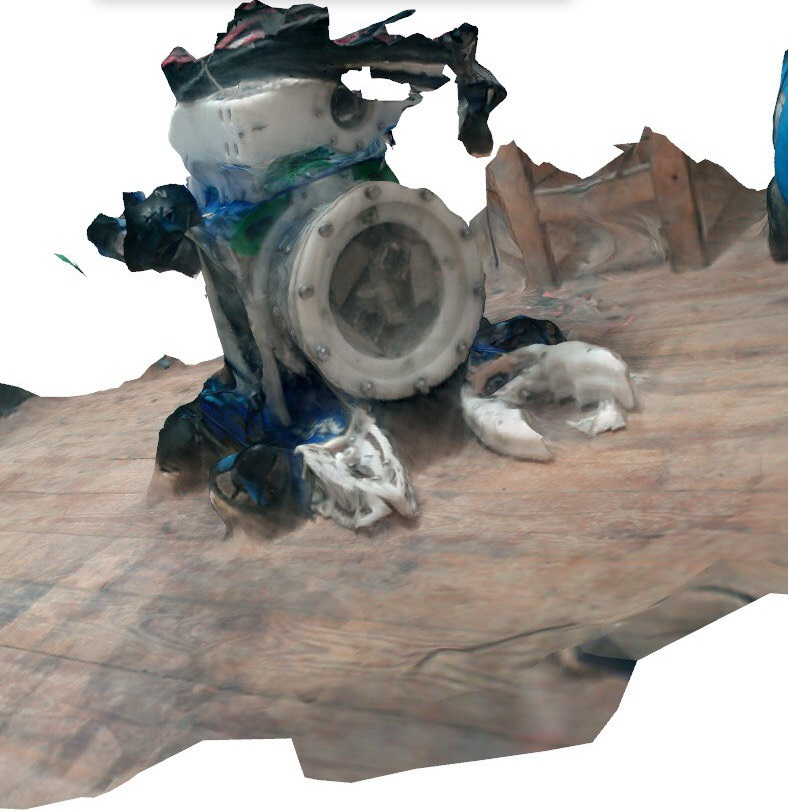
\includegraphics[width=0.27\textwidth]{3d_task_figure2/op1.jpg}};
    \node[above=50pt,text width=100pt,align=center] at (figure3) {Texture Output from different views};
  
    % third figure
    \node[draw, rectangle, blue, fill=blue!20] (figure4) at (8,0) {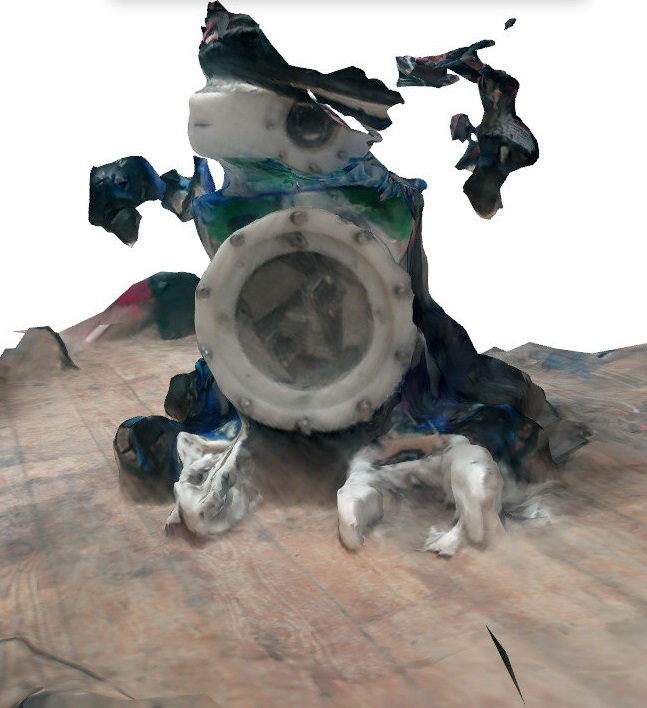
\includegraphics[width=0.27\textwidth]{3d_task_figure2/op2.jpg}};
    
    % Arrow between figures
    \draw[->, line width=1.3pt, blue] (figure1) -- (figure2);
    \draw[->, line width=1.3pt, blue] (figure2) -- (figure3);
    \draw[->, line width=1.3pt, blue] (figure2) -- (figure4);
  \end{tikzpicture}
  \caption{Reconstruction process}
  \label{fig:reconstruction}
  \end{figure}


\subsection*{Dimentions measurement procedures}
To measure the required dimentions, \textbf{Draven} measure a specsified dimention input from user during runtime through a GUI using Streo Camera,
then it can be saved as a reference on the 3D model for other dimentions measurement, as specsified in Figure \ref{fig:measurement}.

\begin{figure}[h]
  \centering
\begin{tikzpicture}
  % First figure
  \node[draw, rectangle, blue, fill=blue!20] (figure1) at (0,0) {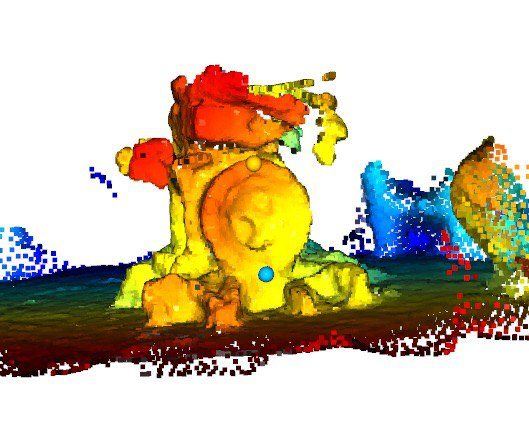
\includegraphics[width=0.25\textwidth]{3d_task_figure1/reference 2.jpg}};
  \node[above=40pt, text width=3cm,align=center] at (figure1) {Known size reference};

  % Second figure
  \node[draw, rectangle, blue, fill=blue!20] (figure2) at (4,0) {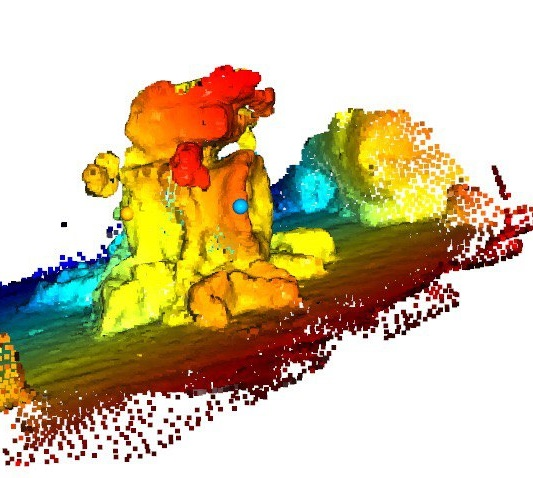
\includegraphics[width=0.25\textwidth]{3d_task_figure1/distance to be measured 2.jpg}};
  \node[above=40pt, text width=100pt,align=center] at (figure2) {Distance to be measured};

  % Third figure
  \node[draw, rectangle, blue, fill=blue!20] (figure3) at (8,0) {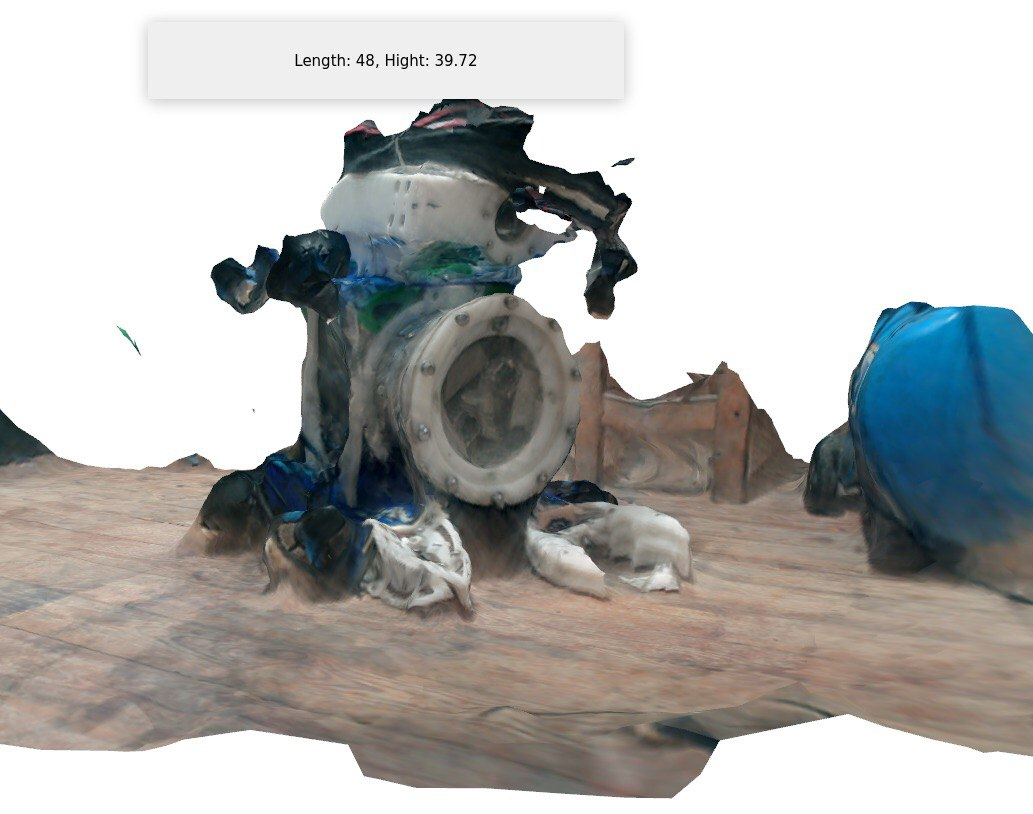
\includegraphics[width=0.32\textwidth]{3d_task_figure1/measurement_output 2.jpg}};
  \node[above=60pt,text width=100pt,align=center] at (figure3) {Measured distance labeled on the model};

  % Arrow between figures
  \draw[->, line width=1.3pt, blue] (figure1) -- (figure2);
  \draw[->, line width=1.3pt, blue] (figure2) -- (figure3);

\end{tikzpicture}
\caption{Measuring process}
\label{fig:measurement}
\end{figure}
\end{document}
